% REMEMBER: You must not plagiarise anything in your report. Be extremely careful.

\documentclass{l4proj}

% put any additional packages here
\usepackage{amsmath}
\usepackage{pdfpages}
\usepackage{float}
\usepackage{cleveref}

\begin{document}

%==============================================================================
%% METADATA
\title{Evaluating the Effectiveness of Extensions to 3D Cross Sections of 4D Geometry in the Teaching and Manipulation of this Geometry}
%\title{An Investigation into Extending a 3D Cross Section of 4D Geometry and Evaluate an Extensions Effectiveness in Teaching Users to Manipulating This Geometry}
\author{Joe Subbiani}
\date{March 18, 2022}

\maketitle

%==============================================================================
%% ABSTRACT
\begin{abstract}
    %Every abstract follows a similar pattern. Motivate; set aims; describe work; explain results.
    %\vskip 0.5em
    %``XYZ is bad. This project investigated ABC to determine if it was! better. ABC used XXX and YYY to implement ZZZ. This is particularly interesting as XXX and YYY have never been used together. It was found that ABC was 20\% better than XYZ, though it caused rabies in half of subjects.''

    Four dimensional space is a mathematical concept that cannot be visualised in its entirety by humans. Several paradigms exist to visualise four dimensional objects in 3D, but a viewer will only be able to see a fraction of a 4D object at one time.
    \vskip 0.5em
    Ray marching over signed distance functions provide a quick method of rendering 3D cross sections of a wide range of primitive 4D shapes.
    3D cross sections of 4D objects provides a platform to develop extended visualisations to provide a user with more information about a 4D object. Such extensions have been explored in other literature. This paper aims to evaluate the effectiveness of a series of extensions to 3D cross sections of 4D objects; each representation providing the user with more information in order to help them interpret and manipulate the object they are handling.
    \vskip 0.5em

    TODO: Results of Experiment
    It was found that ...
    
\end{abstract}

%==============================================================================
%% ACKNOWLEDGEMENTS
\renewcommand{\abstractname}{Acknowledgements}
\begin{abstract}
    I would like to thank my supervisor, Dr. John Williamson for the constant support and advice throughout the project, within and outside of the weekly meetings. Thanks to his guidance and support, I was able to take this project as far as I have, and fully explore the complexities of the fourth dimension.
\end{abstract}
%==============================================================================

% EDUCATION REUSE CONSENT FORM
% If you consent to your project being shown to future students for educational purposes then insert your name and the date below to  sign the education use form that appears in the front of the document. You must explicitly give consent if you wish to do so. If you sign, your project may be included in the Hall of Fame if it scores particularly highly.

% Please note that you are under no obligation to sign  this declaration, but doing so would help future students.

\def\consentname {Dominic Joe Subbiani} % your full name
\def\consentdate {24 January 2022} % the date you agree

\educationalconsent


%==============================================================================
\tableofcontents

%==============================================================================
%% Notes on formatting
%==============================================================================
% The first page, abstract and table of contents are numbered using Roman numerals and are not included in the page count. 

% From now on pages are numbered using Arabic numerals. Therefore, immediately after the first call to \chapter we need the call \pagenumbering{arabic} and this should be called once only in the document. 

% Do not alter the bibliography style.

% The first Chapter should then be on page 1. You are allowed 40 pages for a 40 credit project and 30 pages for a 20 credit report. This includes everything numbered in Arabic numerals (excluding front matter) up to but excluding the appendices and bibliography.

% You must not alter text size (it is currently 10pt) or alter margins or spacing.

%==================================================================================================================================

% IMPORTANT
% The chapter headings here are **suggestions**. You don't have to follow this model if it doesn't fit your project. Every project should have an introduction and conclusion, however. 

%==================================================================================================================================
\chapter{Introduction}

% reset page numbering. Don't remove this!
\pagenumbering{arabic} 

\section{The Fourth Dimension}

The world is described as three dimensional Euclidean space, conventionally referred to as $\mathbb{R}^3$. Three axes, conventionally labeled \(x\), \(y\) and \(z\), define the three degrees of translational freedom an entity can move within. All three axes that make up Euclidean space exist perpendicular to each other. Four dimensional space, conventionally referred to as $\mathbb{R}^4$, is the mathematical concept where a fourth perpendicular axes, conventionally labeled \(w\), exists perpendicular to all of the other three dimensional axes. It is impossible to visualise four dimensions in its entirety and often has to be abstracted to an analogues 3D to 2D example to reason and understand the behaviour of four dimensional entities. 

\section{Opportunities for Exploration}

Handling four dimensional space presents a number of opportunities and challenges that come with the desire to explore, interpret and manipulate higher dimensional objects. The most immediate challenge is that of being able to manipulate a four dimensional object. Rotating an object in a dimensional space greater than two is a non trivial challenge. The most common method of rotation in 3D cannot be extended to higher dimensions. There are several ways in which users can interact with 3D objects; another non-trivial challenge is finding intuitive ways in which a user can manipulate a 4D object through a two dimensional user interface.
\vskip 0.5em
To understand the orientation of an object, a user needs to be able to differentiate similar faces of that object from each other. Colour, patterns and textures can be applied to an object in order to assist in comprehending the current status of an object in comparison to an otherwise visually similar counterpart. An example of this is a cube rotated 90 degrees (\(\frac{\pi}{2}\) radians) and the same cube rotated by 270 degrees (\(\frac{3\pi}{2}\) radians). the un-textured cube would appear be the same despite not being in the same orientation.
\vskip 0.5em
In this paper several methods will be applied in an attempt to provide more information about a four dimensional object. Such methods include: viewing the object from other angles, attempts to visualise the object in its entirety spanning along the \(w\) axis, and abstractions of the rotation of an object in order to help interpret higher dimensional rotations.

\section{Motivation}

% first, motivate then state the general problem clearly. 

Three dimensional space is very neat. There are three degrees of translational freedom expressed by the three axes \(x\), \(y\) and \(z\). There are a further three degrees of rotational freedom that are most commonly expressed as rotations about each axis. 
This supposed tidiness has lead to misconceptions that are so heavily rooted in the average persons understanding of geometry such that nearly every digital 3D system is built upon a mathematically impure foundation. 
%
In the 3D world, these misconceptions do not matter, and the mathematics is still sound. Quaternions, the most common method of controlling or interpreting rotation, is heavily used in gyroscopic devices, interactive digital 3D environments, animation and robotics. More abstract practices such as mathematics and physics, however, need to consider geometry in higher dimensional spaces.
\vskip 0.5em
A variety of fields within science and engineering utilise the visualisation of higher dimensional spaces to tackle a variety of problems. To more intuitively understand a given problem defined in \(n\) dimensional space it is often suitable to reduce the dimensionality of the problem. However, when a problem is reduced to $\mathbb{R}^3$ or $\mathbb{R}^2$ it may become somewhat trivial. Visualisation of 4D objects can often server as the "bridge from the 'trivial cases' to the 'nontrivial cases'", \citep{zhou_visualization_1991}. Such problems that utilise the visualisation of four dimensional space include: Analysis of differential geometry, collision detection, analysis of 3D objects in motion, and scalar-fields in 3D space; among others \citep{zhou_visualization_1991}.
\vskip 0.5em
%
TODO: what is the benefit of trying to teach people about it?\\

\section{Aims}

% wide range of 4 Dimensional shape. variety of ways to display. As such the usability of each representation will be experimentally validated in order to find the most intuitive and effective way to represent higher dimensional shapes. The accuracy of which the user can identify these properties and act accordingly will be measured against the representation being shown to them.

This paper aims to answer questions related to which representation of a 4D object presented through a 3D cross section is the most effective in conveying the properties of four dimensional geometry to a user with limited experience. Which representation is the most effective at representing the surface type of a 4D object? And which representation is more effective at conveying the rotational pose of an object in $\mathbb{R}^4$?
Furthermore, Does a users understanding and ability to manipulate 4D objects increase with practice? And can advantages of each representation be realised and digested by potentially inexperienced users?
\vskip 0.5em
As per the motivation for this project; an effective tutorial has been compiled together in order to explain the foundations of four dimensional geometry. A system to view and interact with 4D objects has be developed in Unity with the capability to showcase a wide variety of 4D shapes using ray marching. Research into intuitive methods of user interaction has been explored, and a system to rotate an object without gimbal lock was employed.
\vskip 0.5em
This paper proposes several extensions to taking a 3D cross section of a four dimensional object. The project evaluation explores what aspects of the geometry emphasised by these extensions are most effective when trying to interpret higher dimensional spaces, and understanding the surface, rotation and pose of a 4D object. 
%
Given a series of tests, a study was conducted that allowed users to manipulate several 4D objects in order to evaluate their understanding of geometry, and compare their understanding against each representation of a 3D cross section. 
Metrics such as time taken, confidence and accuracy were be measured, with each metric being applied to several tests, with each test focusing on a different aspect of geometry in order to evaluate a users understanding of how a cross section of a four dimensional object changes under rotation.

%==================================================================================================================================
\chapter{Background}

\section{Representations of the Fourth Dimension}

There are many ways to represent the fourth dimension. Arguably the most intuitive understanding is that of a 3D cross section. As with how a sphere in $\mathbb{R}^3$ can be considered a stack of infinitely thin circles that vary in size from top to bottom, along the \(z\) axis; a fourth dimensional sphere can be considered a stack of 3D spheres that vary in size as you move across the \(w\) axis.
\vskip 0.5em
The 3D cross section is limited given that only a slice of the shape can be seen at any given time. Stereographic projection attempts to rectify this by allowing a viewer to visualise as much of the shape as their field of view permits. Stereographic projection in $\mathbb{R}^3$ takes a 3D sphere and maps its geometry across a 2D plane. To map another object, for example a cube, its geometry must be projected beforehand onto the surface of a sphere \citep{radiya-dixit_visualizing_2017}. Stereographic projection in $\mathbb{R}^4$ takes the spherical projection of a 4D object, and maps it across a 3D environment. A viewer can stand in the center of the 3D environment and observe the mapped geometry. This approach of interpreting four dimensional space is well suited to virtual reality, however it is complex to interpret in a meaningful way, and abstracting an understanding to lower dimensions is nontrivial.

\subsection{Extensions to the 3D Cross Section}

Through simple discussion with peers, a 3D cross section of a four dimensional object appears to be a far more intuitive concept to grasp compared against stereographic projection. 
%
Given the aims of the project, are to investigate how one may extend a visualisation of a 4D object to provide a viewer with more information in order to assist in their understanding of higher dimensional space, the 3D cross section of a four dimensional world appears most appropriate given it's relative simplicity in using lower dimensional abstractions to assist in understanding higher dimensional geometry.
\vskip 0.5em
An extension to a 3D cross section involves providing the viewer of the object with more information about the object they are dealing with. Several such extensions have already been explored conceptually or even fully developed. 
\vskip 0.5em
Showing several cross sections besides one another, each offset along the \(w\) axis an increased amount is a simple means of trying to provide more information to the user about the entire shape of the object. As shown in the 3D example \cref{fig:exti}: displaying several 2D circles, taken a regular intervals of $\delta$ along the \(z\) axis, that circularly increase and decrease in size provides a viewer with enough information to estimate that the object being displayed is likely a 3D sphere.

\begin{figure}
  \centering
  \begin{subfigure}[b]{0.45\textwidth}
      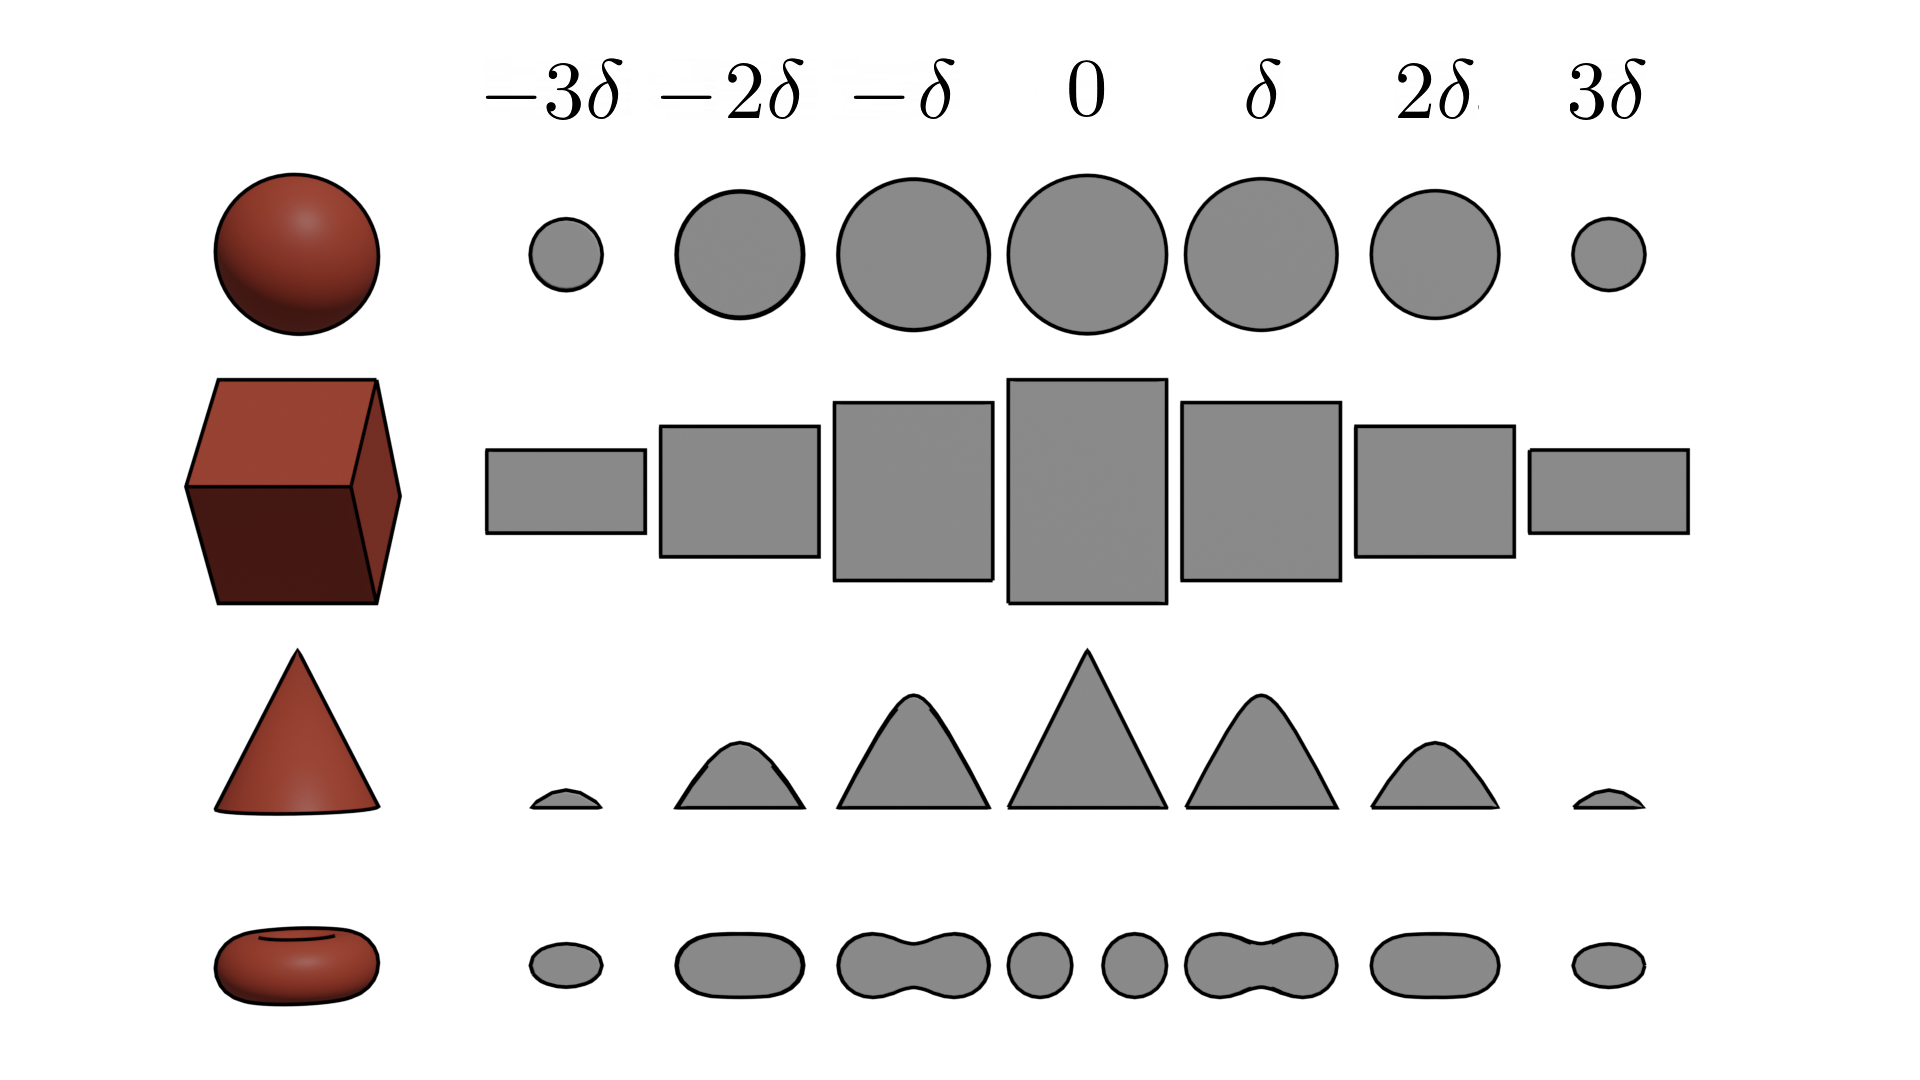
\includegraphics[width=\textwidth]{images/extensions/timeline-delta.png}
      \caption{Several cross sections of 3D objects at $\delta$ intervals along the z axis}
      \label{fig:exti}
  \end{subfigure}
  %
  \begin{subfigure}[b]{0.45\textwidth}
      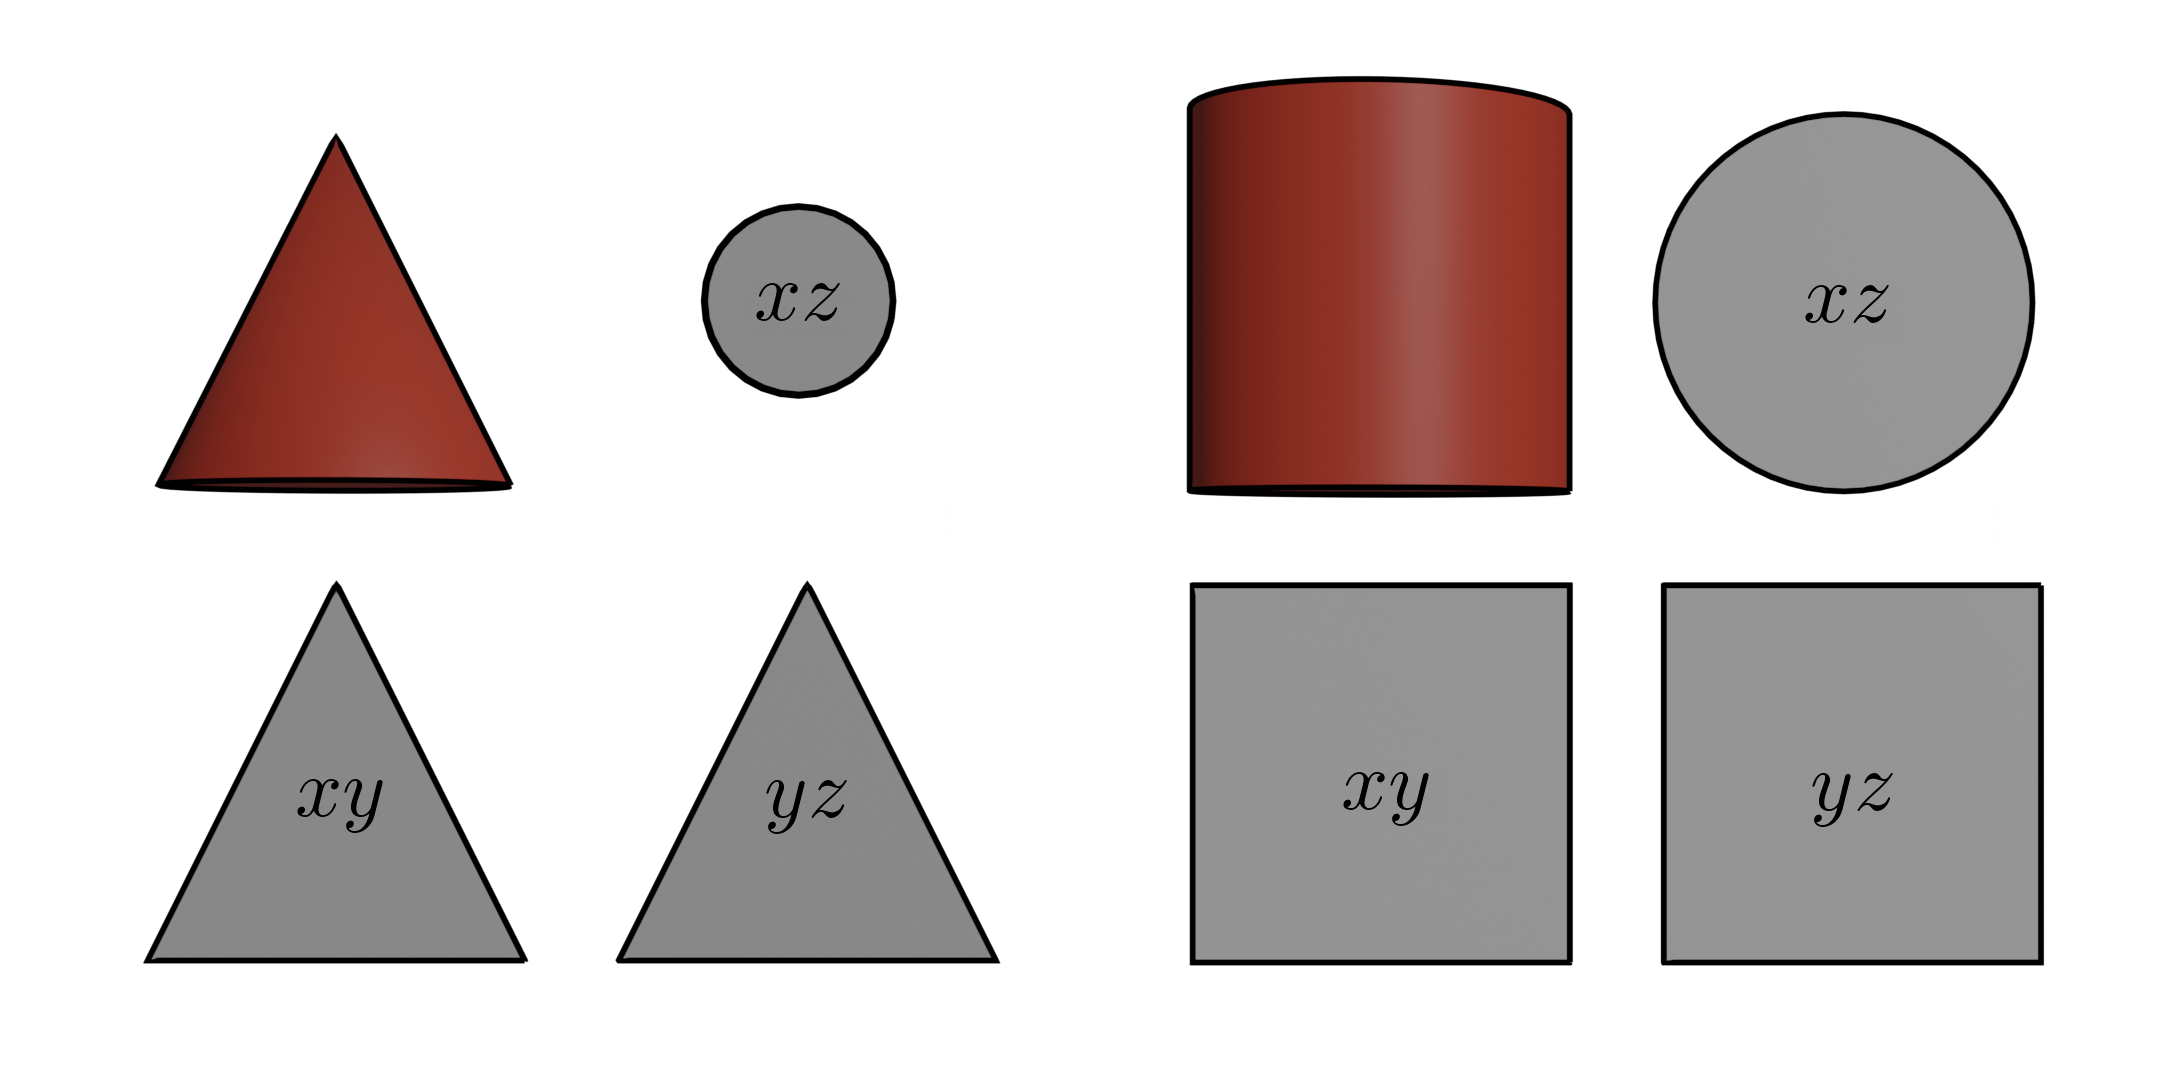
\includegraphics[width=\textwidth]{images/extensions/multi-view.png}
      \caption{Cross sections of a 3D cone and cylinder; where each cross section is taken along the specified plane.}
      \label{fig:exmv}
  \end{subfigure}   
  %
  \caption{Examples of extensions to a 2D cross section of 3D objects.
  }\label{fig:extensions}
\end{figure}

\citet{kageyama_visualization_2015} proposed such a system that displays several cross sections of a 4D object along an ovular path, in order to try and provide a viewer with more information about the object. 
%
By displaying the several cross sections in an ovular path, compared to a linear path, Kageyama was able to display a far greater number of cross sections, allowing for a more detailed view of the four dimensional object in its entirety.
%
Each cross section, as they move further away from the central slice, decreases in size; in order to avoid potential confusion in conveying the idea that travelling across the fourth dimension wraps around, forming a circular path.
%
Scaling each cross section however, can produce some immediate confusion when first viewing an object. For example, taking several cross sections of a 4D cylinder that is extended along the \(w\) axis should produce several 3D spheres of the same size. Kageyama's visualisation will have each of these 3D spheres decrease in size such that a user could likely interpret the shape to be a 3D cross section of a 4D sphere given it exhibits similar scaling behaviour. If a user interacts with the object using the appropriate keys to move across the \(w\) axis, they could observe the lack of change in the size of the central 3D cross section and draw the correct conclusion that it is a cylinder.
Whilst the ovular display does provide a great deal of extra information to a viewer, it is limited by its potential to be obscure when several objects can have similar cross sections.

TODO: classify Kageyama's work
\vskip 0.5em
Another extension which arguably provides the user with more information about an object, is viewing said object from other angles. As shown in the 3D example \cref{fig:exmv}: take a cone that is extended upwards to a point along the \(y\) axis. From the top, a cross section of the object spanning the \(xz\) plane will produce a circle. However a cross section along either the \(xy\) or \(yz\) planes will appear as a triangle.
\vskip 0.5em
\textit{Polyvision}, proposed by \citet{matsumoto_polyvision_2019}, is a virtual reality system to view four dimensional objects from multiple angles to quickly and effectively understand the shape being interacted with.
%
\citet{matsumoto_polyvision_2019} chose to represent 4D objects as wireframes, connecting each vertex of the object by an edge. This is possible when collapsing each vertex of the 4D object to the same three dimensional slice. This is often referred to as the "shadow" of an object. 
A user may view almost all of an object at once using this technique, in comparison to a single 3D slice, whilst potentially offering a more intuitive understanding, although perhaps less information, with comparison to stereographic projection. A disadvantage of a 3D wireframe shadow is with increasingly complex objects, the wireframe cells of the object become more and difficult differentiate with the increase in the number of vertices and edges.
The ability to view the surface of a complex object, such as a 120-cell, likely allows for easier understanding of the geometry compared to the wireframe of its shadow.
%
With the goal of teaching others, \citet{matsumoto_polyvision_2019} restricts interaction to that which we are used to and capable of. Translation, rotation and scaling are restricted to the third dimension. Interaction in $\mathbb{R}^3$, from another perspective in $\mathbb{R}^4$ will change the object in a potentially unexpected way. Whilst the effects of 4D manipulation can be seen in this way, \textit{Polyvision} lacks the ability to directly manipulate an object in 4D space.

TODO: classify Matsumoto's work

\section{Building a 4D Object}

Rendering three dimensional shapes on a 2D screen is an art that has evolved over time and ranges several disciplines. When Tron released in 1982, computers were not powerful enough to render triangle meshes in real time; as is the standard for 3D rendering nowadays. 
Similar films of that era, such as Dune (1984) or Star Wars the Original Trilogy (1977-1983) often used a mix of practical effects and physically modifying the film, using techniques such as rotoscoping and double exposure. The team behind tron, however, opted to take advantage of machines to do some heavy lifting. In-spite of the technological limitations the team were able build a system to combine and render simple but smooth primitive objects. They used a system called Ray Marching \citep{sheppard_tron_2010}.
\vskip 0.5em
Today, it is standard to use triangle meshes to build and even render complex models in real time; and not just for film, but for real time interactive media such as video games.
A mesh consists of vertices, edges and faces. A vertex being a point on the surface of an object that edges connect to. A face is formed by a closed loop of edges. Generally, a face will be made up of three vertices and three edges, creating the most simple 2D shape: A triangle; which form a part of the surface of a 3D mesh.

\subsection{Mesh Based Rendering}

Both \citet{bosch_n-dimensional_2020} and \citet{tianli_4d_2018} have developed real time interactive systems which display four dimensional objects using mesh based rendering. As illustrated by \citet{tianli_4d_2018}, 4D shapes are made up of cells, similar to how a 3D mesh is made up of faces. As with a face in a 3D mesh being constructed of triangles (the most basic 2D shape), a 4D mesh is constructed of the most basic cell, a tetrahedron. A tetrahedron is made up of four triangles defined by faces, vertices and edges. The pentachoron, also known as a hyper-tetrahedron or a 5-cell, is the most primitive 4D object besides potentially the hyper-sphere. The mesh of a pentachoron consists of 5 tetrahedral sub-meshes (cells). A sub-mesh in this instance refers to a 3D mesh used to build a 4D object, in the same way a 2D net of faces can build a 3D shape.
\vskip 0.5em
Mesh based rendering allows the creation of very complex higher dimensional objects. \citet{bosch_n-dimensional_2020} built a novel game engine implementing four dimensional rigid body dynamics, as well as the rendering of a four dimensional world. 
On the other hand, \citet{tianli_4d_2018} used the readily available Unity game engine to construct a hyper-cube and hyper-tetrahedron, demonstrating the flexibility of existing software built for two and three dimensions.
\vskip 0.5em
There are two main drawbacks to mesh based rendering: The time taken to construct 4D objects, and the complexity of translating four dimensional geometry to 3D. 
%
Simple 4D Platonic solids \citep{parker_things_2014} such as the hyper-tetrahedron (5-cell), hyper-cube (8-cell) and hyper-octahedron (16-cell) are fairly straightforward. Developing complex shapes such as a the hyper-dodecahedron (120-cell) or the hyper-iscosahedron (600-cell) becomes a complex and time consuming task. 
This complexity only increase when trying to develop curve faced shapes such as a hyper-sphere, torus or cone, which are smooth. Smooth geometry generally requires hundreds of vertices as well as smooth surface shading that only add to computational load and development time.
\vskip 0.5em
In order to render a three dimensional slice of a four dimensional object, an algorithm must be employed such that a point along an edge that connects two vertices of a 4D object can be found, and connected by edges to all other points lying on the same four dimensional hyperplane that sit along the edge connect other 4D vertices of the same object. This is a fairly complex task, and only gets more complex when calculating what faces of the slice of the object to render to produce a cohesive three dimensional slice. \citet{tianli_2d_2018} demonstrates how to find the cross section of an object and the problems associated with it.

\subsection{Ray Marching Shaders}

Ray march based rendering was initially developed due to limitations in real time rendering, as a way to combine easy to define primitive objects into more complex shapes. Despite advancements in rendering capabilities, allowing even low-end computers to render complex mesh based geometry in real time, ray marching has not lost its place in the world. 
Whilst ray marching has often thought to evolved into ray tracing, the foundation of photorealistic rendering, signed distance fields (SDFs), the core of ray marching, are still heavily used in volumetric geometry, meta-ball geometry, collision detection and ray marched shaders.
An SDF is a function that describes a signed distance to a surface relative to a point in space. \citet{quilez_distance_nodate} lists several SDFs for primitive objects as well as functions that can be applied to them.

% Ray marching Diagrams
\begin{figure}[H]
  \centering
  \begin{subfigure}[b]{0.45\textwidth}
      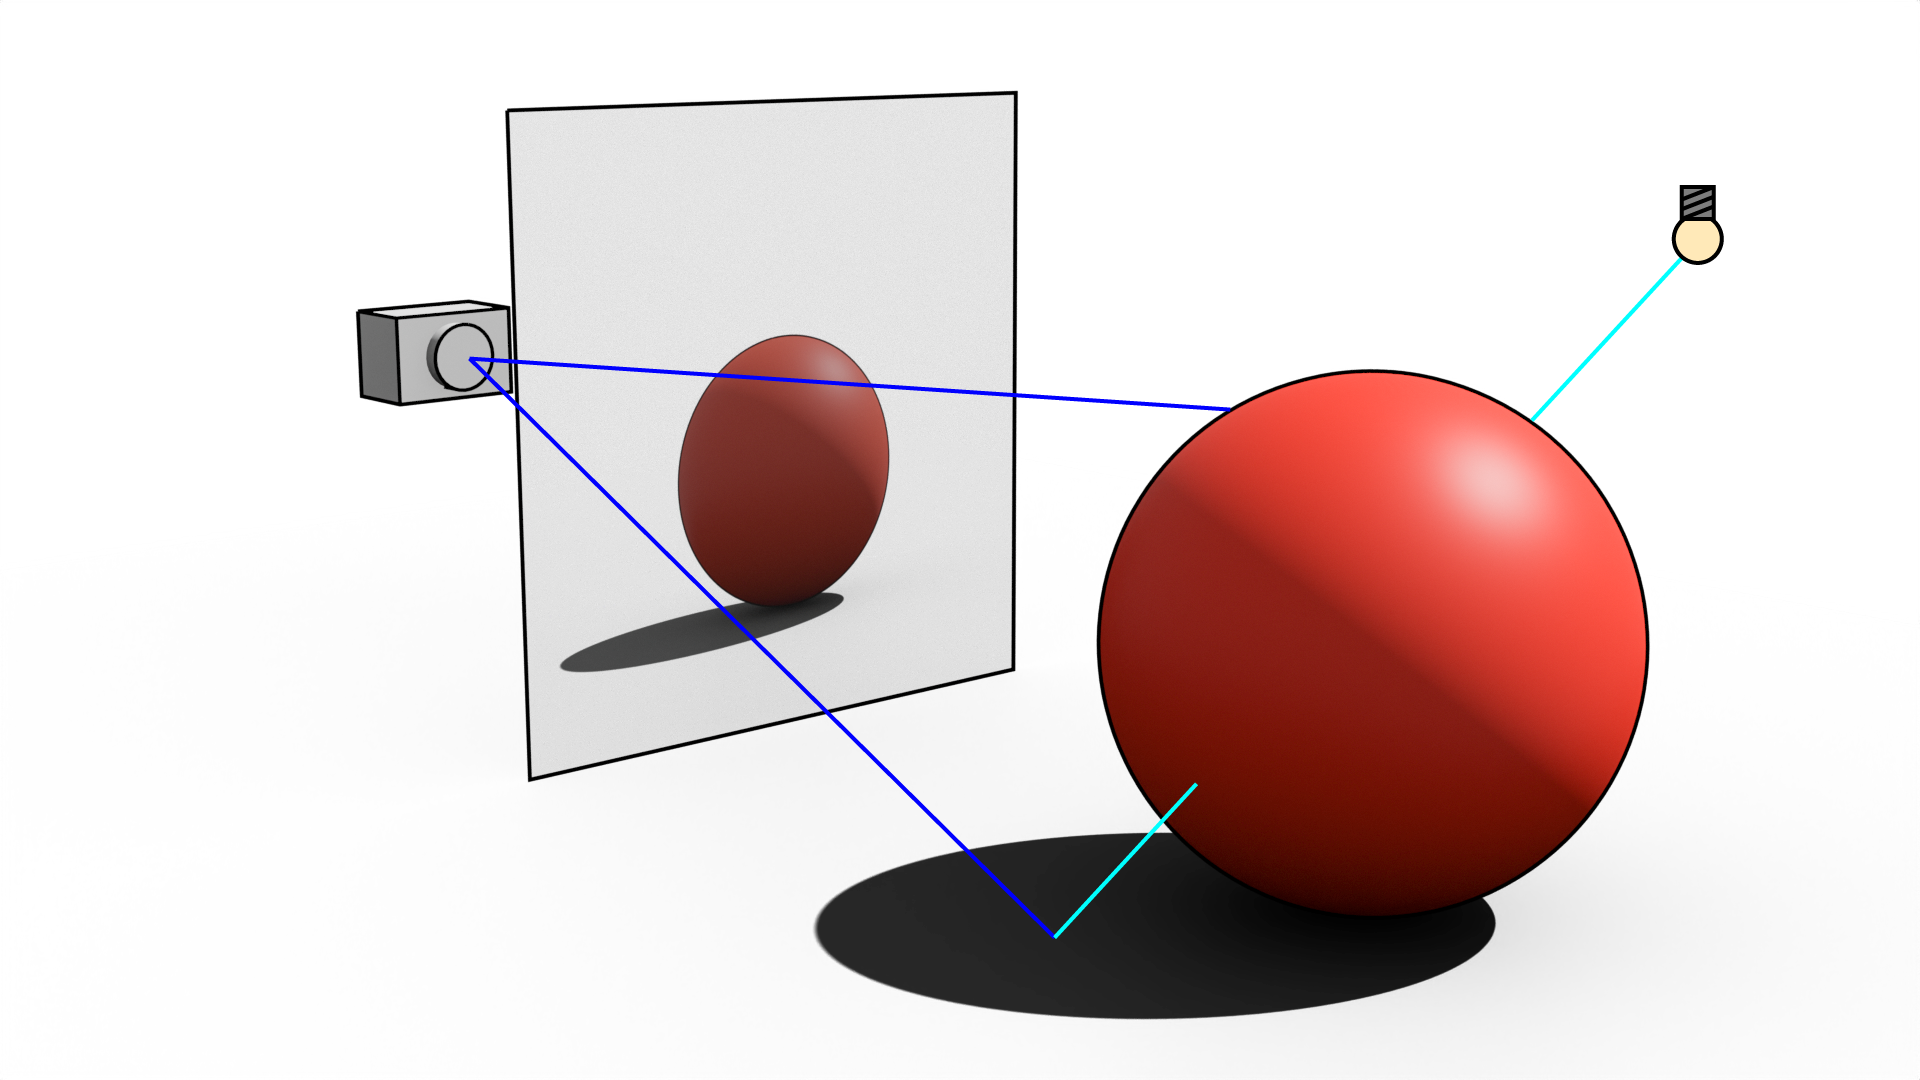
\includegraphics[width=\textwidth]{images/raymarching/raymarch_ai.png}
      \caption{Ray marching to produce an image}
      \label{fig:rmcast}
  \end{subfigure}
  %
  \begin{subfigure}[b]{0.45\textwidth}
      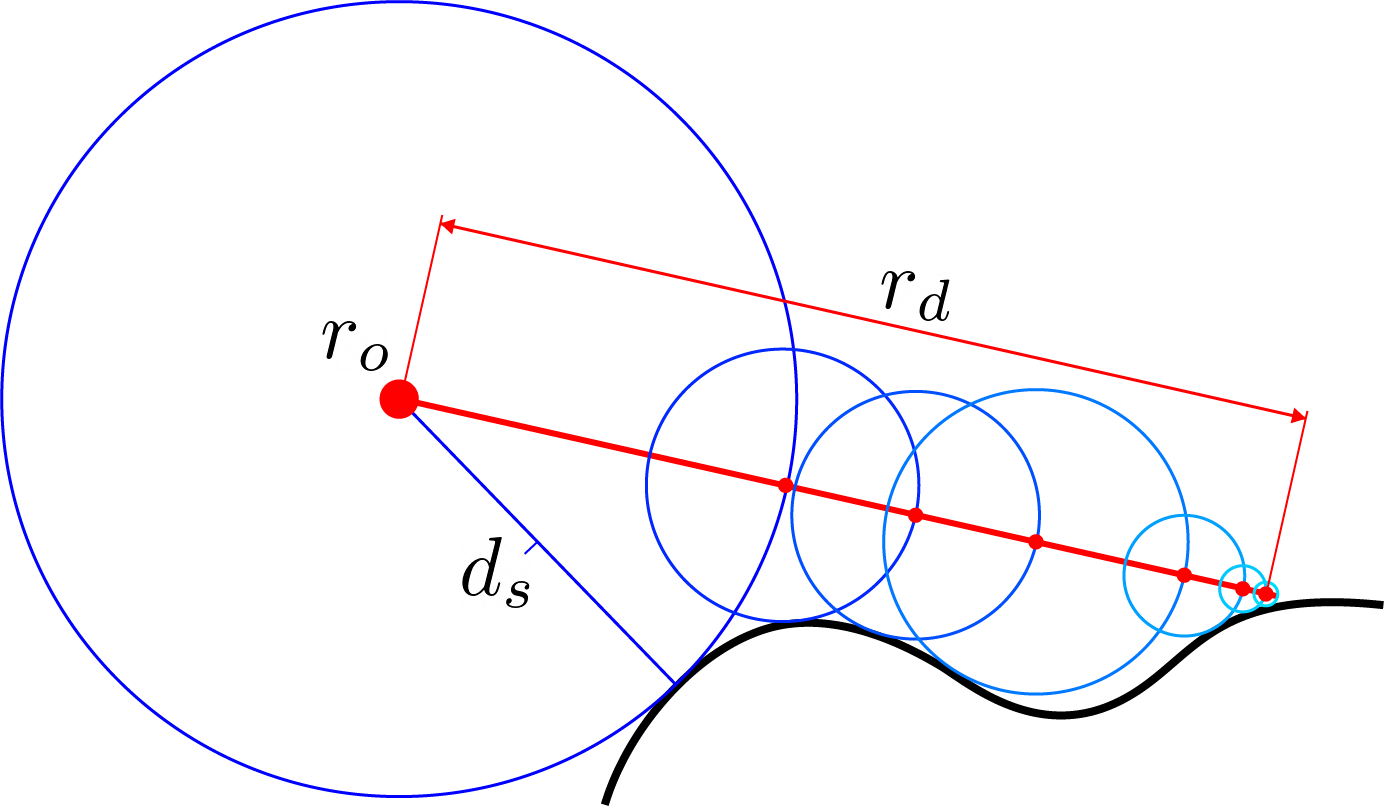
\includegraphics[width=\textwidth]{images/raymarching/algorithm_ai.png}
      \caption{Ray marching algorithm}
      \label{fig:rmalg}
  \end{subfigure}   
  %
  \caption{Ray marching. \subref{fig:rmcast} shows how each pixel of an image is coloured by casting a ray from the camera in the direction of the pixel and reading the surface of any defined geometry. 
  \subref{fig:rmalg} shows the process of a single ray marching towards a surface, given a an origin point and a direction as described in \cref{alg:raymarch}.
  }\label{fig:raymarch}
\end{figure}
%
% Ray marching Algorithm
\begin{algorithm}[H]
  \DontPrintSemicolon
  
  \KwData{\\
    \quad $r_o$ the origin of a ray.\;
    \quad $r_d$ the direction of a ray.\;
    \quad $MAX\_STEPS$ the maximum number of iterations.\;
    \quad $MAX\_DIST$ the maximum distance from the ray origin.\;
    \quad $SURF\_DIST$ the smallest distance from a surface before deciding not to step any further.\;
    \quad $SDF(p)$ given a point $p$ along the ray, return the distance to the nearest surface.\;
  }
  \KwResult{\\
    \quad $ d_o $ The distance from the ray origin along the ray path.
  }
  \Begin{
      $ d_o \longleftarrow 0 $\;
      $ d_s \longleftarrow \infty $\;
      \For{$ i < MAX\_STEPS $}
      {
          $ p \longleftarrow r_o + d_o \cdot r_d$\;
          $ d_s \longleftarrow SDF(p) $\;
          $ d_o \longleftarrow d_s + d_o $\;
          \If{$d_s < SURF\_DIST \textbf{ or } d_o > MAX\_DIST$}
          {
              break\;
          }
      }
  }
\caption{The ray marching algorithm}\label{alg:raymarch}
\end{algorithm}
\pagebreak

Ray marching (\cref{alg:raymarch}, \cref{fig:raymarch}) is the processes of calculating the colour of each pixel on a screen by casting a ray from an origin point in the direction of a pixel to colour the pixel based on the distance to a mathematically defined geometric surface. Given an origin point and a direction, the algorithm takes the distance to the nearest surface and then marches forward by that distance to map out the surface detail. \citep{the_art_of_code_ray_2018}.
\vskip 0.5em
%
Whilst less intuitive and approachable than mesh based rendering, there are active communities which strive to build interesting or complex geometry using these mathematical expressions in conjunction with ray marching. \textit{Shadertoy}, developed by \citet{quilez_shadertoy_2013}, is a web based platform that allows anyone to create and experiment with shader based geometry.
\vskip 0.5em
A significant advantage over mesh based rendering is the ability to render a 3D cross section of a 4D object with minimal effort. The SDF of a 4D object taken over three dimensional space will produce the SDF equivalent to the cross section of the same object in a given hyper plane along the \(w\) axis.
It is not novel to ray march over primitive 4D objects such as the hyper cube or hyper sphere. Often, primitive SDFs taken over $\mathbb{R}^3$ can be easily extended to $\mathbb{R}^4$; and this is the case for many of the SDFs developed by \citet{quilez_distance_nodate}. Other 4D geometry on the other hand needed to be derived from scratch. 

\section{Rotating a 4D Object}

In $\mathbb{R}^3$ there are three degrees of rotational freedom. As there are three axes, the method of rotating an object has commonly been considered as rotating about an axis. However, in $\mathbb{R}^4$ there are six degrees of rotational freedom, despite there only being four axes. Instead, rotation must be considered as a rotation about a plane formed by two axes. Therefore the six planes of rotation in $\mathbb{R}^4$ are \(xy\), \(xz\), \(yz\), \(xw\), \(yw\) and \(zw\).

\subsection{The Problems with Rotation}

Rotating an object in $\mathbb{R}^2$ is somewhat trivial. Given a vector $v_{xy}$ rotating an angle $\theta$ about an origin point within the \(xy\) plane, the vector will follow a circular path dictated by the following 2D rotation matrix:
% 2D Rotation Matrix
\begin{equation}
    v_{xy}' = v_{xy}\begin{bmatrix}
      cos \theta & - sin \theta \\
      sin \theta & cos \theta
    \end{bmatrix},
\end{equation}
%
Rotating an object in a space greater than two dimensions immediately becomes a nontrivial problem due to its non-commutativity. In dimensions greater than $\mathbb{R}^2$, rotation matrices can be composed into a homogeneous rotation matrix. Multiplying a vector with a such a matrix will produce a rotated vector, but doing so will likely encounter gimbal lock. Gimbal lock occurs when rotating an object considers each plane of rotation as independent from one another. As a result, if a particular plane becomes parallel with another, a degree of rotation is lost and the vector being rotated will not change as expected.
\vskip 0.5em
Introducing the quaternion: The quaternion is an extension of the complex number system. A quaternion has 4 components: \(x\), \(y\) and \(z\) which describe the axis of rotation, and \(w\) which describes the amount of rotation. Quaternions do not suffer from gimbal lock and can be applied to each other to perform several rotations in series.
\vskip 0.5em
Quaternions have a problem: They consider rotations as a rotation about an axis. As discussed by \citet{bosch_lets_nodate}, axial rotations are not appropriate as a generalised method of rotation across dimensions. For example, you would not consider a 2D object rotating within two dimensions as rotating about the \(z\) axis. It makes far more sense to stay within $\mathbb{R}^2$ and rotate about the \(xy\) plane.

\subsection{Geometric Algebra and The Rotor}
\label{ga_and_rotor}

Geometric Algebra, often referred to as Clifford Algebra, is a field of mathematics describing vector space. Vector space is populated by multivectors, graded by their vector components. Most notably, multivectors are defined by their associative, distributive and anti-commutative properties \citep{baker_maths_nodate}.
A grade zero multivector is a scalar number. a grade one multivector is just a vector. Grade two multivectors are known as bivectors, which build the foundation for the rotor. A trivector is a grade 3 multivector forming a parallelepiped from 3 vectors. Finally in $\mathbb{R}^4$ there is what is known as a pseudo-scalar.
\vskip 0.5em
A bivector $b_{ab}$ is made up of two vectors \(a\) and \(b\), and has, alongside its orientation in space defined by it's vector components, two important properties: The direction of rotation, from \(a\) to \(b\), and an area, dictated by the parallelogram formed by its two vector components as illustrated by \citet{slehar_clifford_2014}. A bivector in the reverse direction, i.e from \(b\) to \(a\) fulfills the anti-commutative property such that $b_{ba} = -b_{ab}$. 
% TODO: Wedge Product similar to Cross Product
\vskip 0.5em
As mentioned above, a rotation should be considered as a rotation about a plane. A bivector defines the plane for a vector to rotate about. As demonstrated by \citet{mathoma_geometric_2017}, a rotor can rotate a vector following the principle that a double reflection forms a rotation \citep{mathoma_geometric_2016-2}.
\vskip 0.5em
In a given vector space greater than $\mathbb{R}^2$, a multivector greater than grade zero can be projected onto the vector space basis blades. A basis blade is a the plane formed parallel to two perpendicular axes. The \(xy\) blade is often referred to as $e_x \wedge e_y$ or $e_{xy}$ or sometimes $e_{01}$. Therefore a bivector in $\mathbb{R}^3$ can be decomposed into three projections onto the $e_{xy}$, $e_{xz}$ and $e_{yz}$ planes; and a bivector in $\mathbb{R}^4$ can be decomposed into 6 elements. To decompose a bivector into its projections, the outer (or wedge) product of the two vectors which form said bivector can be used.
\vskip 0.5em
It is possible to multiply multivectors using the geometric product; a combination of the inner and outer product. Multiplying a vector \(v\) by a rotor \(R\) and it's reverse \(R^\dagger\) will rotate vector about the bivector component of the rotor. Order matters here.
%
\begin{equation}
  \label{eq:sanwhich_a}
    v' = R v R^\dagger,
\end{equation}
%
Rotors can also be multiplied using the geometric product. This will produce a new rotor. Therefore two rotors; $R_a$ and $R_b$, can be composed as shown in \cref{eq:sanwhich_b} to rotate a vector \(v\) and produce a rotated vector \(v'\).
%
\begin{equation}
  \label{eq:sanwhich_b}
  v' = R_a R_b v R_a^{\dagger} R_b^{\dagger}
   = (R_a R_b) v (R_a R_b)^{\dagger}
   = R_{ab}^{} v R_{ab}^{\dagger}
\end{equation}
%
The angle of rotation is dictated by a scalar component of the rotor, similar to the \(w\) component of a quaternion. 
As shown by \citep{bosch_code_nodate}, the quaternion and the 3D rotor are very similar in concept. The rotor, unlike the quaternion, has the advantage of not having to leave the dimensionality of the vector in order to rotate the vector, allowing it to be used in \(n\) dimensions.

\section{Interaction and Direct Manipulation}

\subsection{Methods of Interaction in 3D}

local, grab ball driven

global, swipe gestures (often multi-touch)

\citep{shoemake_arcball_1994}\\
\citep{hinckley_usability_1997}\\
\citep{balakrishnan_rockinmouse_1997}

\subsection{Methods of Interaction in 4D}

\citep{murata_interactive_2000}\\
\citep{kageyama_keyboard-based_2005}

\section{Teaching and Evaluation}

In order to evaluate the effectiveness of each extension to a 3D cross section of a 4D object, as stated in the aims of this investigation, a participant should have an understanding of what four dimensional geometry is, and how it behaves.
For this investigation, it was a priority to ensure this complex mathematical topic can be well communicated to individuals with little-to-no experience of higher dimensional space, prior to conducting the experiment of the representations of the 4D geometry. \textit{The van Hiele Model of Geometric Thinking}, \citep{safrankova_van_2012}, Theorises that their are five levels of understanding geometry, where a student will progress from one level to the next. The levels of understanding include: Visualisation, Analysis, Abstraction, Deduction and Rigor, numbered 0 to 4 respectively.
Level 0 focuses on the identification and recognition of geometry using simple language. The properties that define a geometry need not be identified.
Level 1: students begin basic analysis and identification of geometry, without a need for proofs.
Level 2: students create meaningful definitions and are able to justify and reason their understanding of geometry.
Level 3: students are able to provide deductive geometry proofs, showing their understanding of formal definitions and theorems.
Level 4: students have an understanding of several proofs and can comprehend Euclidean and non-Euclidean geometry.
\vskip 0.5em
\citet{safrankova_van_2012} outlines the five stages of the learning process that should be covered when teach a student about geometry in order to comprehensively cover the material in such a way that a student will understand it; as outlined in the van Hiele model.
\textit{Information inquiry} is where students receive the relevant material and discover the structure of the information they are handling. At this stage a teacher should use familiar language to help a student relate what they already understand to the new material.
\textit{Guided or directed orientation} deals with the exploration of relationships within the material. A teacher may suggest activities enabling students to recognise the properties of a new concept. Discussion is encourage between the student and the teacher to assist in discovering relationships between properties of the material.
\textit{Explanation or Explication}: Here, students formulate what they have discovered. New terminology is introduced whilst the student shares their opinion on what relationship is discovered. Here a teacher can ensure the correct terminology is being used.
The \textit{Free orientation} stage allows for students to solve more complex tasks independently to master the network of relationships within the content. In this stage a student may develop their understanding of the properties of geometry as well as develop their understanding of the relationships between geometry in a variety of scenarios.
Finally, \textit{Integration} involves the student summarising what they have learned. No new material is presented in this stage.
\vskip 0.5em
For the purposes of this experiment, only levels 0 to 2 of \textit{The van Hiele Model of Geometric Thinking} will be explored. A rule of the model is that a student may not progress to level \(N\) without having first tackled level $N-1$. 
In order to best evaluate the effectiveness of an extension to the 3D cross section of a 4D object, a participant of the investigation should understand the geometry they are working with to some degree.
Unfortunately, given the limited time to conduct the investigation, and an individual experiment, participants will not be able to sufficiently progress through each level, whilst also covering each of the five stages of the learning process. 
To provide a participant with the best possible foundations for understanding four dimensions, tutorials and question and answer sessions before and after each stage in the experiment were be conducted. The experiment was designed to try follow the structure of the five stage learning process as closely as would allow. This is expanded upon more in the experimental design section (\cref{experimental_design}) of this paper.

%==================================================================================================================================
\chapter{Analysis and Requirements}

\section{Problem Specification}

The core of this project focuses on the development of a system capable of rendering several different types of four dimensional objects, and be able to view these objects through a series of extensions to the 3D cross section in order to evaluate their effectiveness in teaching potentially inexperienced users about complex geometry.
\vskip 0.5em
For a successful investigation, a focus was placed on the visualisation of 4D geometry, as well as how users learn and interpret this geometry. It is important that the experiment was to be clear and concise. Both quantitative and qualitative metrics were obtained. The experiment needed tests probing a participant on the surface type, behaviour under rotation and identification of the rotational pose of an object in $\mathbb{R}^4$ given different representations of an objects cross section.

\section{Limitations}

The scope of the project is limited by two main factors: The time that can be spent on development, and the quantity to quality ratio of experimentation. 
The project is primarily separated into three components: Research, development and experimentation. The development phase took the most time with so many areas for exploration. Such areas include the creation, stable rotation, and manipulation of 4D geometry. To evaluate the effectiveness of the representations that need to be developed however, plenty of time needs to be put aside to plan and run appropriate experiments.
Experimentation is, more often than not, limited by the number of participants that choose to be involved. To encourage the greatest number of potential participants to enroll in the experiment, the time commitment and effort cannot be so great that it deters them. Alongside the conscious effort to sign up, the experiment cannot run for such a period of time that it may effect a participants performance. As such, the amount of data that can be collected in one sitting was to be maximised within a limited time frame.

\section{The Framework}
\label{requirements_framework}

The project was developed in the Unity game engine using ray marching shaders. Unity is readily available to anyone for free; and allows for quick and simple application deployment for web based hosting using WebGL and HTML5. 
Given the COVID-19 pandemic at the time of the experiment, online hosting was an important consideration to allow for a more accessible experiment in a world where people are having to self isolate. Not only does this allow for a participants safety, but the size of the audience can be increased. Online hosting reduces the commitment a participant has to make, making the experiment more appealing. Time to commute and costs of travel that potential participants would otherwise have to make, now no longer factor into the considerations made by a potential participant when signing up for the experiment.
\vskip 0.5em
Ray marching was used rather than mesh based rendering given its comparative ease. Several 4D shapes can be written fairly quickly using ray marching. Although complex geometry with defined faces, such as the 120-cell is a struggle to write using ray marching, render curved geometry using mesh based rendering requires the development of a smooth shading rendering effect. Furthermore, implementing a rendering of the 3D cross section of a 4D object is comparatively trivial using ray marching. To render the three dimensional cross section of a 4D mesh is yet another system to develop that would require more time and research. 
Generally, ray marching is more suitable to this project in exploring primitive geometry in $\mathbb{R}^4$, and allows for more time to be spent on research and development into stable rotation and manipulation of 4D geometry, and the creation of a cohesive investigation.

\section{Prioritisation of Requirements Using MoSCoW}

MoSCoW is a prioritisation technique used in project planning. The purpose of MoSCoW is to separate the requirements of a project into four levels of priority: Must have, Should have, Could have and Won't have. This process may be revisited several times during a projects development lifecycle; different requirements are often re-prioritised based on project progress or a change in direction.

\subsection*{Must Have}

The following requirements are necessary in order to conduct a successful evaluation and were compiled and refined throughout the projects development:

A system must be developed that is capable of rendering 4D shapes. As such, several 4D shapes must be created. 
In order to test a persons understanding, of the 4D shapes that are to be developed, they must not all be immediately distinguishable from one another. For example, a hyper-cube and a hyper-sphere will never look similar to each other, whereas, the 3D cross section of a 4D hyper-cone in a particular pose will look identical to the 3D cross section of a 4D hyper-sphere.
\vskip 0.5em
The aims of the project focus on the development of several extensions to the 3D cross section in order to find what extensions are better for conveying the complexities of 4D geometry to potentially novice users. Therefore, several extensions to the 3D cross section of four dimensional space should be developed. The extensions to the 3D cross section may take inspiration from the literature mentioned earlier, and attempt to improve upon or emphasise the components of their work that are relevant to this investigation.
\vskip 0.5em
To distinguish the faces of shapes, the objects will need to be coloured such that given two objects in a different pose, both objects can be distinguished from one another even if their surface shape appears identical. 
\vskip 0.5em
In order to prepare participants for the experiment, an introductory tutorial video will need to be assembled to teach and explain them about the complexities and features of the fourth dimension. This tutorial video must cover the behaviour of geometry in $\mathbb{R}^4$, with appropriate references to the similarities when reducing three dimensional space to a two dimensional cross section. Moreover, the video must explain rotation in four dimensions, as well as an explanation for the behaviour that occurs when rotating an object outside of the dimensions it is being viewed within. The video must have relevant diagrams and animations to appropriately depict the behaviour of 4D shapes in such a way that it will be immediately relatable to the following experiment.
%\vskip 0.5em
\pagebreak

Before running the experiments, the tests must be completed and evaluated several times by myself, with some preliminary research with a small group of peers to ensure the functionality of the system is as expected, and any restraints such as time limits are within acceptable bounds.
\vskip 0.5em
Finally the experiment must have multiple stages of testing to evaluate a persons understanding of the several aspects of geometry. The experiment must not last such a long time that it affects the participants performance. To appropriately evaluate a persons understanding alongside the effectiveness of a representation, qualitative data must be collected from the participant, about their understanding, including open and closed questions.

\subsection*{Should Have}

Whilst not a necessity, the following requirements would enhance the investigation, allowing the further exploration of the four dimensional world.

"Free orientation", as stated by \citet{safrankova_van_2012}, is an important aspect in a students learning and understanding of the definition and behaviour of geometry. In order for a participant to master the complexities of geometry in $\mathbb{R}^4$ they should be able to handle 4D objects directly.
Evaluating a participants understanding of a shape, its surface and its behaviour under rotation can be conducted without directly interacting with or manipulating an object, a system should be developed to allow a participant to directly interact with 4D objects in order to perceive, first hand, the effect they have on the cross section o the geometry.
For direct manipulation in four dimensions, a 4D Rotor must be implemented to allow for stable interaction, without fear of gimbal lock.

\subsection*{Could Have}

Given the limitations, although it would be nice to include, the following requirements are the lowest priority. The requirements will be explored, but are not necessary to conduct the investigation and will likely not be refined to a satisfactory degree.

It would be desirable to implement a series of tools allowing for intuitive interaction of 4D geometry, and such methods of interaction will be experimented with. The experiments, however, will only implement one method of rotation for the experiment, given the investigation focuses on the ways to enhance the cross section of 4D space, rather than how to manipulate these objects. Therefore, it is of minimal priority to develop several methods of rotation, although during the research and development phase, several methods of interaction will be explored.

%==================================================================================================================================
\chapter{Design}

requirements for teaching
 - match up with van-hiele model

 information inquiry - VIDEO
 - students receive information and discover structure
 - well known language

guided or directed orientation - VIDEO
 - deal with tasks to explore relationships
 - teacher that suggests activities enabling students to recognise properties of a new concept
 - relationships are discovered and discussed
   - encourage discussion

explanation or explication - DISCUSSION AFTER VIDEO
 - student formulate what they have discovered and new terminology is introduced
 - share opinion on relationships discovered
   - encourage discussion
 - teacher ensures correct terminology - more useful than familiarity with concept

free orientation - MOST IMPORTANT FOR THIS PROJECT
 - student solves more complex tasks independently
 - master network of relationships in material
 - know properties but develop understanding of relationships in various situations

integration - DISCUSSION BETWEEN VIDEO AND EXPERIMENT
 - student summarises what they have learnt
 - do not present new material in this phase
 - summary of what has been learned

OTHER STUFF
 - explain 4D space, why it cannot be visualised
 - explain 4D rotation in relation to 2D and 3D rotation

\section{Tutorial}



\section{Experiment}
\label{experimental_design}


requirements for testing

 - be able to understand the shapes
 - be able to interpret the rotation of a shapes
 - be able to manipulate a shape

%==================================================================================================================================
\chapter{Implementation}

\section{Building 4D Objects With Ray Marching}

As stated in \cref{requirements_framework}, the combination of Unity and ray marching shaders were used to develop and render three dimensional objects cross sections of four dimensional objects.
Ray marching over signed distance functions in Unity has often been used within art and game development communities. 
The first phase of implementing a system to render four dimensional objects was to form a foundation: implement a three dimensional ray marcher in Unity \citep{the_art_of_code_writing_2019}. 
The ray marching algorithm (\cref{alg:raymarch}) casts a ray from an origin pointer towards a pixel on the screen, to determine how to colour this pixel. The algorithm takes a signed distance function (SDF) which defines the surface relative to an origin point, given a point \(p\) along the ray. 
To summarise the basics of SDFs, \cref{lst:sdSphere} shows a signed distance function written in GLSL for a 3D sphere, with radius \(r\). 
The center of the sphere is described as an offset from the origin. To apply this to the point \(p\), along the ray, the opposing translation must be applied. Using \(p\), the distance to the surface is calculated. Given $r=0$ the distance returned by the function would be the distance to the center of the sphere. By subtracting the radius from the distance to the center of the object, a radius is described around the point defining surface of the sphere.
Therefore, the SDF returns the distance to the surface of a sphere, defined by a radius and a point offset from the origin.
\vskip 0.5em
%
\begin{lstlisting}[language=glsl, caption={The signed distance function for a sphere in $\mathbb{R}^3$ with a center at $(1,0,0)$, and radius $r$}, label=lst:sdSphere]
  float sdSphere( float3 p, float r )
  {
      p -= float3(1,0,0);
      return length(p)-r;
  }
\end{lstlisting}

The 3D ray marching shader written in Unity defines two vectors describing the ray origin and the hit position of the ray. These vectors are used to define the ray origin and ray direction for each pixel, to calculate what the shader should render.
When extending the ray marcher to four dimensions, the majority of the process was enabling the algorithm and its components, such as the SDF, to take 4D vectors (\texttt{float4}), rather than a 3D (\texttt{float3}). Given the components of the shader describing the ray origin and direction existed along the same slice of four dimensions, only a single 3D slice of the four dimensional space was taken and rendered, giving us the 3D cross section.
\vskip 0.5em
With the standard ray marcher implemented the shader can only interpret whether a ray hits a surface or not. The only information of a 3D shape that can be gathered from this binary value will be its 2D shadow. In order to render a 3D component of the object, we need light and shadows. 
Two basic methods of shading include angle dependant light falloff and shadows cast by other objects obstructing a light source \cref{lst:rm_light}. 
A surface normal is a vector that is perpendicular to a point on the surface and can be used to measure the angle of the surface relative to another vector. 
Using the surface normal an angle dependant light falloff can be implemented such that a surfaces light value will be lower if the difference between the surface normal and the vector to the light source is higher.
A shadow cast by on to a surface can be taken by ray marching from a surface in the direction of the light source to check if there is another surface obstructing the path. If there is, the surfaces light value can be lowered.

\begin{lstlisting}[language=glsl, float, caption={Given a light position \texttt{lightPos}, shade the surface based on the fall off angle and cast a shadow, if a surface is obstructing another surface from the light source}, label=lst:rm_light]
float4 GetNormal(float4 p)
{
    float2 e = float2(0.01, 0);

    float4 n = GetDist(p) - float4( 
        GetDist(p-e.xyyy),
        GetDist(p-e.yxyy),
        GetDist(p-e.yyxy),
        GetDist(p-e.yyyx)
    );
    return normalize(n);
}

float GetLight(float4 p, float4 lightPos)
{
    //angle dependant fall off
    float4 lv = normalize(lightPos-p);
    float4 n  = GetNormal(p);
    float  light  = clamp(dot(n,lv), 0., 1.);

    //shadow
    float4 so = p + n * SURF_DIST * 2.; //shadow origin
    float4 sd = normalize(lightPos-so); //light direction
    float d = Raymarch(so, sd);
    if( d < length(lightPos-p) ) light *= 0.1;

    return light;
}
\end{lstlisting}

\subsection{Derivation of 4D Shapes}

Of the 3D SDFs derived by \citet{quilez_distance_nodate} and \citet{the_art_of_code_ray_2019}, the sphere, box, and capsule were fairly trivial to translate directly to four dimensional space.
A 4D hyper sphere takes a radius, with the surface spanning equally along all four axes.
A 4D box takes a 4D vector where each component describes the height, width, depth and length of the box along each of the four axes respectively.
Similar to how the sphere subtracts the radius from the distance to the origin point, the box subtracts the 4D vector containing the dimensions of the box. 
To produce flat faces for each side of the box without the distance function stepping passed the surface, the vector is combined with the zero vector using a boolean intersection, with the use of \texttt{max(a, b)}. The derivation is best described by \citet{the_art_of_code_ray_2019}.
%TODO: interior distance and 
Finally a 4D capsule can be described as a line connecting two points, \(A\) and \(B\), and the line is given a thickness via a radius. Just as with the sphere, the radius spans in all four dimensions.
\vskip 0.5em
The torus is an interesting shape; two variations were developed for this project.
A 3D torus can be described by a major radius, $r_1$ and a minor radius $r_2$. $r_1$ is the main ring of the torus, and $r_2$ is the thickness of this ring - its radius.
When you take a 2D slice of a 3D torus it may appear as a pair of circles a distance $2(R_1 - R_2)$ apart as shown in \cref{fig:exti}. 
Similar to the cross section of a sphere, it makes sense to have the radius $r_2$ of the two circles expand into the fourth dimension, such that a 3D cross section of a four dimensional torus may appear as a pair of 3D spheres.
Alternatively, consider a four dimensional torus with three radii: $r_1$, $r_2$ and $r_3$. Similar to how the 3D torus can be described as a circle with a thickness, a 4D torus with three radii describes a circle defined by radius $r_1$, with radius $r_2$ surrounding the circle that is given a thickness defined by the radius $r_3$. 
Essentially this produces a circle with a torus sweeping across its path. Therefore, a 3D cross section of this torus may appear as two tori with a major radius of $r_2$ and minor radius of $r_3$ separated by a distance of $2(r_1 - (r_2 + r_3))$.
\vskip 0.5em
The 3D cross section of a 4D cone would in some instances appear as a 3D cone, and in other instances appear as a 3D sphere, in the same way a 3D cones' 2D cross section may in some cases appear as a triangle or a circle (\cref{fig:exmv}). 
The cone SDFs developed by \citet{quilez_distance_nodate} and others define the cone by its height and slope. This approach did not extend well to 4D, and defining an instance of a cone was rather unintuitive.
The SDF for the cone implemented takes a height and the radius at the base of the cone. This approach extends well to $\mathbb{R}^4$, as rather than a defining the cone as a surface function of angle and height, it defines the slice of the cone at any given cross section.
\vskip 0.5em
Of the shapes defined thus far, the 4D box is the only shape with edges, meaning it would obviously stand out against the other curved surfaces. 
A 4D tetrahedron, also known as a pentachoron (5-cell), was created to present another platonic solid, showcasing the boxes similarities with other shapes.
The SDF of plane can be defined by its normal vector. For example, The SDF of a plane that spans $xy$ in $\mathbb{R}^3$ would simply be \texttt{p.y}.
A tetrahedron is made up of 4 triangular faces, each opposing one of it's four vertices. The SDF for a tetrahedron can be defined by four vectors describing the normal of each face. These vector can actually be taken as the coordinates fo the four vertices making up the shape. Each of these vectors defines the SDF of a plane parallel to each face of the tetrahedron respectively. By taking the boolean intersection of these planes using \texttt{max(a, b)}, the SDF for a tetrahedron is produced.
The SDF for a tetrahedron also takes a parameter $s$, used to scale the tetrahedron. Subtracting $s$ from the distance to the surface, the surface is effectively brought further from the center, similar to the radius of a sphere.
Constructing a pentachoron is done in a near identical way, just five vertices are considered rather than four.

\section{Extending 3 Dimensional Cross Sections: \\Representing 4D Objects}

The signed distance function referenced in the ray marching algorithm defines the scene to be rendered. In this function, several other SDFs can be referenced to render several objects at once. To render several SDFs at once, each function may be combined using a boolean union: taking the minimum distance between two or more objects using \texttt{min(a, b)}.
\vskip 0.5em


timeline: simple - ellyptical version
 - ellypitcal adds more information, but not as intuitive as straight line\\
onionskin - similar to timeline, but not very intuitive for users unfamiliar with 4D\\
multi-view: polyvision\\
abstraction of 4D rotation using 3D rotation - does not extend well to n dimensions unlike all other propositions

\section{Rotation of a 4D Vector}

As discussed in \cref{ga_and_rotor}, geometric algebra provides a platform for stable rotation of a vector in $\mathbb{R}^4$ without gimbal lock. 
The rotor is straightforward to work with when considering the abstract multivectors as single entities. Implementing a rotor in code, on the other hand, is a more complex task. 
A rotor is made up of three multivectors: A scalar, a bivector and a pseudo-scalar. To perform arithmetic operations on non-scalar multivectors, they must be broken down into projections. 

TODO: Explain Projections + Figure - vector and bivector
\label{fig:vec_proj}
\label{fig:bivec_proj}

In $\mathbb{R}^4$ a grade 1 multivector (Vector) \(a\) can be broken down into four components. Each component is the vector projected onto one of the four axes (\cref{eq:vec_components}). One of the four projections is therefore a scalar value describing the vectors distance along an axis (\cref{fig:vec_proj}).
%
\begin{equation}
  \label{eq:vec_components}
  a = a^x + a^y + a^z + a^w
\end{equation}
%
In $\mathbb{R}^4$ a grade 2 multivector (Bivector) \(b\) is described by its area and orientation in space. A bivector can be broken down into six components, where each component is the bivectors projection onto each plane that can be taken from the four axes (\cref{eq:bivec_components}). A projection of the bivector onto a plane is a scalar value equivalent to the area of the projected bivector which will be less than or equal to the area of the bivector (\cref{fig:bivec_proj}).
%
\begin{equation}
  \label{eq:bivec_components}
  b = b^{xy} + b^{xz} + b^{xw} + b^{yz} + b^{yw} + b^{zw}
\end{equation}
%
As stated above, a rotor in $\mathbb{R}^4$ is comprised of a grade 0 multivector (Scalar) \(s\), a bivector and a grade 4 multivector (pseudo-scalar) \(p\) (\cref{eq:rotor_components}). The bivector defines the plane of rotation to rotate the vector about. The scalar describes how much to rotate the vector by. The pseudo-scalar is required for 4D rotation to normalise the rotor and ensure stable rotation; without it the vector may rotate unpredictably or increase/decrease in size.
%
\begin{equation}
  \label{eq:rotor_components}
  R = s + b + p^{xyzw} = 
  s + b^{xy} + b^{xz} + b^{xw} + b^{yz} + b^{yw} + b^{zw} + p^{xyzw}
\end{equation}
%
\citep{bosch_4d_2011}

\citet{bosch_code_nodate} 


initial manual derivation

sympy and galgebra: Listing \cref{lst:rotor_derivation}\\
equation to rotate vector: Equation \cref{eq:rotate_vec}\\
equation to rotate rotor: Equation \cref{eq:rotate_rotor}

\section{Methods of Rotation}

\subsection{Swipe Based Input - Rotation About The Global Axes}

intuitive\\
does not define "how rotated" 4D axes are relative to the local coordinates of the shape

\subsection{4D Grab Ball - Rotation About The Local Axes}

idea\\
progress\\
why it failed

\section{Texturing Ray Marched Objects}

normal based projection

\section{Building the Experiment}

\subsection{}

\subsection{Data Collection}

SimpleJSON \citep{bunny83_simplejson_nodate}

Email - challenges\\
Copy \& Paste - challenges

%==================================================================================================================================
\chapter{Evaluation} 

\section{Aims} 

\section{Experimental Design}

\subsection{Preliminary Research}

what is the best way to explain concepts\\
try teach some friends the basics and see what explanations work best

the best ways to teach people about geometry\\
 - reference that paper about 5 stages or something

between users experiment
 - test user with every representation

\subsection{Repeated Preliminary Experiments}

build system\\
test it\\
improvements\\

Need to provide clear explanations of concepts early on

provide time to play with object before tests to learn controls and behaviour

\subsection{Tasks and Parameters}

shape match\\
 - all shapes\\
 - diffuse texture - patterns give it away\\
rotation match\\
 - not diffuse texture and no sphere - no surface imperfections and can be impossible to tell if certain rotations occuring\\
 - 1-2 4D rotations and occasionally 3d rotations\\
pose match\\
 - randomly oriented match shape

random order of representations

\subsection{Limitations}

\section{Results}

\citep{glen_jaccard_2022}

\subsection{Quantitative Results}


\subsection{Qualitative Results}


%==================================================================================================================================
\chapter{Conclusion}    
Summarise the whole project for a lazy reader who didn't read the rest (e.g. a prize-awarding committee).
\section{Guidance}
\begin{itemize}
    \item
        Summarise briefly and fairly.
    \item
        You should be addressing the general problem you introduced in the
        Introduction.        
    \item
        Include summary of concrete results (``the new compiler ran 2x
        faster'')
    \item
        Indicate what future work could be done, but remember: \textbf{you
        won't get credit for things you haven't done}.
\end{itemize}

%==================================================================================================================================
%
% 
%==================================================================================================================================
%  APPENDICES  

\begin{appendices}

\chapter{Appendices}

%\begin{itemize}
%\item
%  Copies of ethics approvals (required if obtained)
%\item
%  Extensive tables or figures that are too bulky to fit in the main body of the report, particularly ones that are repetitive and summarised in the body.
%\item 
%  Outline of the source code (e.g. directory structure), or other architecture documentation like class diagrams.
%\item 
%  User manuals, and any guides to starting/running the software.
%\end{itemize}

% Rotor Product Derivation
\begin{lstlisting}[language=python, caption={
  Rotor4 product derivation using Geometric Algebra in python: \\
  Rotor4-Vector rotation using double reflection; producing \cref{eq:rotate_vec}.\\
  Rotor4-Rotor4 product to apply a 4D Rotor to another 4D Rotor; producing \cref{eq:rotate_rotor}.
  }, label=lst:rotor_derivation]
  from sympy import symbols
  from galgebra.ga import Ga
  from galgebra.printer import Format
  
  Format(Fmode = False, Dmode = True)
  
  s4coords = (x,y,z,w) = symbols('x y z w', real=True)
  s4 = Ga('e', g=[1,1,1,1],
  coords=s4coords)
  
  def rotate_vector():
    # Vector
    a = s4.mv('a','vector')

    # Rotor
    s = s4.mv('s', 'scalar')
    b = s4.mv('b','bivector')
    p = s4.mv('p', 'pseudo')
    rotor = s + b + p
  
    (rotor * a * rotor.rev()).Fmt(3)
  
  def rotor_rotor_product
    # Rotor A
    a_s = s4.mv('a_s', 'scalar')
    a_b = s4.mv('a_b','bivector')
    a_p = s4.mv('a_p', 'pseudo')
    rotor_a = a_s + a_b + a_p
  
    # Rotor B
    b_s = s4.mv('b_s', 'scalar')
    b_b = s4.mv('b_b','bivector')
    b_p = s4.mv('b_p', 'pseudo')
    rotor_b = b_s + b_b + b_p
  
    (rotor_a * rotor_b).Fmt(3)
  
\end{lstlisting}

\begin{equation} 
  \begin{aligned}
    \label{eq:rotate_vec} 
  & + \Big( 2 a^{w} b^{xw} s + 2 a^{w} b^{xy} b^{yw} + 2 a^{w} b^{xz} b^{zw} + 2 a^{w} b^{yz} p^{xyzw} \\
  & \quad - a^{x} {\left ( b^{xw} \right )}^{2} - a^{x} {\left ( b^{xy} \right )}^{2} - a^{x} {\left ( b^{xz} \right )}^{2} + a^{x} {\left ( b^{yw} \right )}^{2} + a^{x} {\left ( b^{yz} \right )}^{2} + a^{x} {\left ( b^{zw} \right )}^{2} - a^{x} {\left ( p^{xyzw} \right )}^{2} + a^{x} s^{2} \\
  & \quad - 2 a^{y} b^{xw} b^{yw} + 2 a^{y} b^{xy} s - 2 a^{y} b^{xz} b^{yz} + 2 a^{y} b^{zw} p^{xyzw} \\
  & \quad - 2 a^{z} b^{xw} b^{zw} + 2 a^{z} b^{xy} b^{yz} + 2 a^{z} b^{xz} s - 2 a^{z} b^{yw} p^{xyzw} \Big) \boldsymbol{e}_{x} \\
  %
  & + \Big( - 2 a^{w} b^{xw} b^{xy} - 2 a^{w} b^{xz} p^{xyzw} + 2 a^{w} b^{yw} s + 2 a^{w} b^{yz} b^{zw} \\
  & \quad - 2 a^{x} b^{xw} b^{yw} - 2 a^{x} b^{xy} s - 2 a^{x} b^{xz} b^{yz} - 2 a^{x} b^{zw} p^{xyzw} \\
  & \quad + a^{y} {\left ( b^{xw} \right )}^{2} - a^{y} {\left ( b^{xy} \right )}^{2} + a^{y} {\left ( b^{xz} \right )}^{2} - a^{y} {\left ( b^{yw} \right )}^{2} - a^{y} {\left ( b^{yz} \right )}^{2} + a^{y} {\left ( b^{zw} \right )}^{2} - a^{y} {\left ( p^{xyzw} \right )}^{2} + a^{y} s^{2} \\
  & \quad + 2 a^{z} b^{xw} p^{xyzw} - 2 a^{z} b^{xy} b^{xz} - 2 a^{z} b^{yw} b^{zw} + 2 a^{z} b^{yz} s \Big) \boldsymbol{e}_{y} \\
  %
  & + \Big( - 2 a^{w} b^{xw} b^{xz} + 2 a^{w} b^{xy} p^{xyzw} - 2 a^{w} b^{yw} b^{yz} + 2 a^{w} b^{zw} s \\ 
  & \quad - 2 a^{x} b^{xw} b^{zw} + 2 a^{x} b^{xy} b^{yz} - 2 a^{x} b^{xz} s + 2 a^{x} b^{yw} p^{xyzw} \\
  & \quad - 2 a^{y} b^{xw} p^{xyzw} - 2 a^{y} b^{xy} b^{xz} - 2 a^{y} b^{yw} b^{zw} - 2 a^{y} b^{yz} s \\
  & \quad + a^{z} {\left ( b^{xw} \right )}^{2} + a^{z} {\left ( b^{xy} \right )}^{2} - a^{z} {\left ( b^{xz} \right )}^{2} + a^{z} {\left ( b^{yw} \right )}^{2} - a^{z} {\left ( b^{yz} \right )}^{2} - a^{z} {\left ( b^{zw} \right )}^{2} - a^{z} {\left ( p^{xyzw} \right )}^{2} + a^{z} s^{2} \Big) \boldsymbol{e}_{z} \\
  %
  & + \Big( - a^{w} {\left ( b^{xw} \right )}^{2} + a^{w} {\left ( b^{xy} \right )}^{2} + a^{w} {\left ( b^{xz} \right )}^{2} - a^{w} {\left ( b^{yw} \right )}^{2} + a^{w} {\left ( b^{yz} \right )}^{2} - a^{w} {\left ( b^{zw} \right )}^{2} - a^{w} {\left ( p^{xyzw} \right )}^{2} + a^{w} s^{2} \\
  & \quad - 2 a^{x} b^{xw} s + 2 a^{x} b^{xy} b^{yw} + 2 a^{x} b^{xz} b^{zw} - 2 a^{x} b^{yz} p^{xyzw} \\
  & \quad - 2 a^{y} b^{xw} b^{xy} + 2 a^{y} b^{xz} p^{xyzw} - 2 a^{y} b^{yw} s + 2 a^{y} b^{yz} b^{zw} \\
  & \quad - 2 a^{z} b^{xw} b^{xz} - 2 a^{z} b^{xy} p^{xyzw} - 2 a^{z} b^{yw} b^{yz} - 2 a^{z} b^{zw} s \Big) \boldsymbol{e}_{w}  
  \end{aligned}
\end{equation}

\begin{equation}
  \begin{aligned}[t]   
    \label{eq:rotate_rotor}
  & + \left ( - a^{xw}_{b} b^{xw}_{b} - a^{xy}_{b} b^{xy}_{b} - a^{xz}_{b} b^{xz}_{b} - a^{yw}_{b} b^{yw}_{b} - a^{yz}_{b} b^{yz}_{b} - a^{zw}_{b} b^{zw}_{b} + a^{xyzw}_{p} b^{xyzw}_{p} + a_{s} b_{s}\right )  \\  
  & + \left ( - a^{xw}_{b} b^{yw}_{b} + a^{xy}_{b} b_{s} - a^{xz}_{b} b^{yz}_{b} + a^{yw}_{b} b^{xw}_{b} + a^{yz}_{b} b^{xz}_{b} - a^{zw}_{b} b^{xyzw}_{p} - a^{xyzw}_{p} b^{zw}_{b} + a_{s} b^{xy}_{b}\right ) \boldsymbol{e}_{x}\wedge \boldsymbol{e}_{y} \\  
  & + \left ( - a^{xw}_{b} b^{zw}_{b} + a^{xy}_{b} b^{yz}_{b} + a^{xz}_{b} b_{s} + a^{yw}_{b} b^{xyzw}_{p} - a^{yz}_{b} b^{xy}_{b} + a^{zw}_{b} b^{xw}_{b} + a^{xyzw}_{p} b^{yw}_{b} + a_{s} b^{xz}_{b}\right ) \boldsymbol{e}_{x}\wedge \boldsymbol{e}_{z} \\ 
  & + \left ( a^{xw}_{b} b_{s} + a^{xy}_{b} b^{yw}_{b} + a^{xz}_{b} b^{zw}_{b} - a^{yw}_{b} b^{xy}_{b} - a^{yz}_{b} b^{xyzw}_{p} - a^{zw}_{b} b^{xz}_{b} - a^{xyzw}_{p} b^{yz}_{b} + a_{s} b^{xw}_{b}\right ) \boldsymbol{e}_{x}\wedge \boldsymbol{e}_{w} \\  
  & + \left ( - a^{xw}_{b} b^{xyzw}_{p} - a^{xy}_{b} b^{xz}_{b} + a^{xz}_{b} b^{xy}_{b} - a^{yw}_{b} b^{zw}_{b} + a^{yz}_{b} b_{s} + a^{zw}_{b} b^{yw}_{b} - a^{xyzw}_{p} b^{xw}_{b} + a_{s} b^{yz}_{b}\right ) \boldsymbol{e}_{y}\wedge \boldsymbol{e}_{z} \\  
  & + \left ( a^{xw}_{b} b^{xy}_{b} - a^{xy}_{b} b^{xw}_{b} + a^{xz}_{b} b^{xyzw}_{p} + a^{yw}_{b} b_{s} + a^{yz}_{b} b^{zw}_{b} - a^{zw}_{b} b^{yz}_{b} + a^{xyzw}_{p} b^{xz}_{b} + a_{s} b^{yw}_{b}\right ) \boldsymbol{e}_{y}\wedge \boldsymbol{e}_{w} \\ 
  & + \left ( a^{xw}_{b} b^{xz}_{b} - a^{xy}_{b} b^{xyzw}_{p} - a^{xz}_{b} b^{xw}_{b} + a^{yw}_{b} b^{yz}_{b} - a^{yz}_{b} b^{yw}_{b} + a^{zw}_{b} b_{s} - a^{xyzw}_{p} b^{xy}_{b} + a_{s} b^{zw}_{b}\right ) \boldsymbol{e}_{z}\wedge \boldsymbol{e}_{w} \\ 
  & + \left ( a^{xw}_{b} b^{yz}_{b} + a^{xy}_{b} b^{zw}_{b} - a^{xz}_{b} b^{yw}_{b} - a^{yw}_{b} b^{xz}_{b} + a^{yz}_{b} b^{xw}_{b} + a^{zw}_{b} b^{xy}_{b} + a^{xyzw}_{p} b_{s} + a_{s} b^{xyzw}_{p}\right ) \boldsymbol{e}_{x}\wedge \boldsymbol{e}_{y}\wedge \boldsymbol{e}_{z}\wedge \boldsymbol{e}_{w}  \end{aligned}
\end{equation}

%Questionnaire
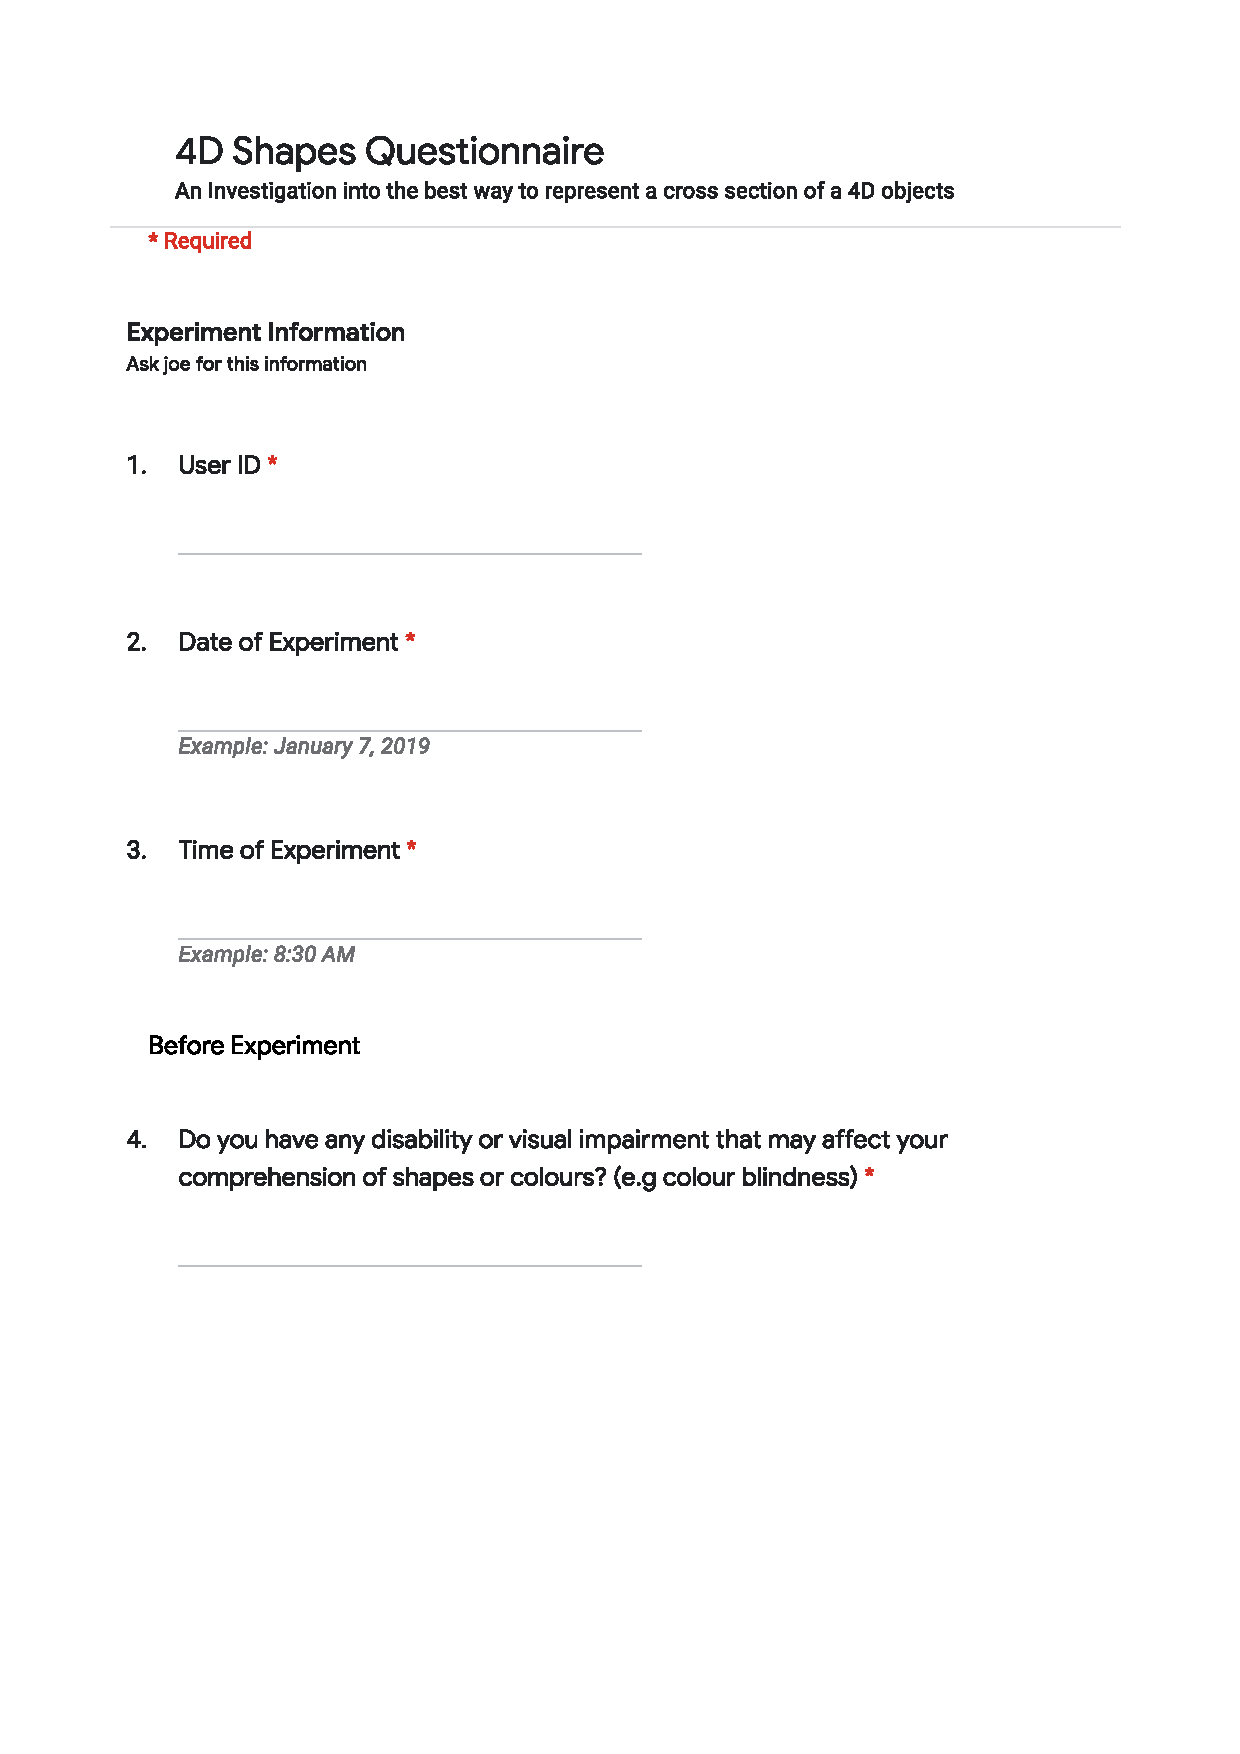
\includepdf[width=1.1\linewidth, pages={1-4}]{images/4d_shapes_questionnaire.pdf}

\end{appendices}

%==================================================================================================================================
%   BIBLIOGRAPHY   

% The bibliography style is abbrvnat
% The bibliography always appears last, after the appendices.

\bibliographystyle{abbrvnat}

\bibliography{l4proj}

\end{document}
